\section{A case study in clustering}\label{section:examples}

\subsection{\(k\)-means clustering}

The following examples act as a form of validation for EDO, and also highlight
some of the nuances in its use. The objective of these examples is to use the
proposed method to reproduce some known results about the clustering of data in
the absence of any external forces, and to examine how clustering algorithms are
typically evaluated. In particular, the focus will be on the well-known
\(k\)-means (Lloyd's) algorithm. Clustering was chosen as it is a
well-understood problem that is easily accessible \-- especially when restricted
to two dimensions. The \(k\)-means algorithm is an iterative, centroid-based
method that aims to minimise the `inertia' of the current partition, \(Z =
\left\{Z_1, \ldots, Z_k\right\}\), of some dataset \(X\):
\begin{equation}
    I(Z, X) := \frac{1}{|X|} \sum_{j=1}^{k} \sum_{x \in Z_j} {d(x, z_j)}^2
    \label{eq:inertia}
\end{equation}

A full statement of the algorithm to minimise~(\ref{eq:inertia}) is given
in~\ref{app:kmeans}. 

This inertia function is taken as the objective of the \(k\)-means algorithm,
and is used for evaluating the final clustering. This is particularly true when
the algorithm is not being considered an unsupervised classifier where accuracy
may be used~\cite{Huang1998}. With that, the first example will use this inertia
as the fitness function in EDO.\ That is, to find datasets which minimise \(I\).

For the purposes of visualisation, EDO is restricted to the space containing
only two-dimensional datasets, i.e.\ \(C = \left((2, 2)\right)\). In addition to
this, all columns are formed from uniform distributions where the bounds are
sampled from the unit interval. Thus, the only family in \(\mathcal{P}\) is:
\begin{equation}
    \mathcal{U} := \left\{U(a, b)~|~a, b \in [0, 1]\right\}
\end{equation}

The remaining parameters are as follows: \(N~=~100\), \(R~=~(3, 100)\),
\(M~=~1000\), \(b~=~0.2\), \(l~=~0\), \(p_m~=~0.01\), and shrinkage is excluded.
Figure~\ref{fig:small-inertia-50} shows an example of the fitness (above) and
dimension (below) progression of the evolutionary algorithm under these
conditions up until the \(50^{th}\) epoch.

There is a steep learning curve here; within the first 50 generations an
individual is found with a fitness of roughly \(10^{-10}\) which could not be
improved on for a further 900 epochs. The same quick convergence is seen in the
number of rows. This behaviour is quickly recognised as preferable and was
dominant across all the trials conducted in this work. This preference for
datasets with fewer rows is expected given that \(I\) is the sum of the mean
error from each cluster centre. With that, when \(k\) is fixed \textit{a
priori}, reducing the number of points in each cluster (i.e.\ the terms of the
second summation) quickly reduces the mean error of that cluster and thus the
value of \(I\).

\addtocounter{figure}{1}
\begin{figure}[htbp]
    \ContinuedFloat%
    \centering
    \begin{tabular}{c}
        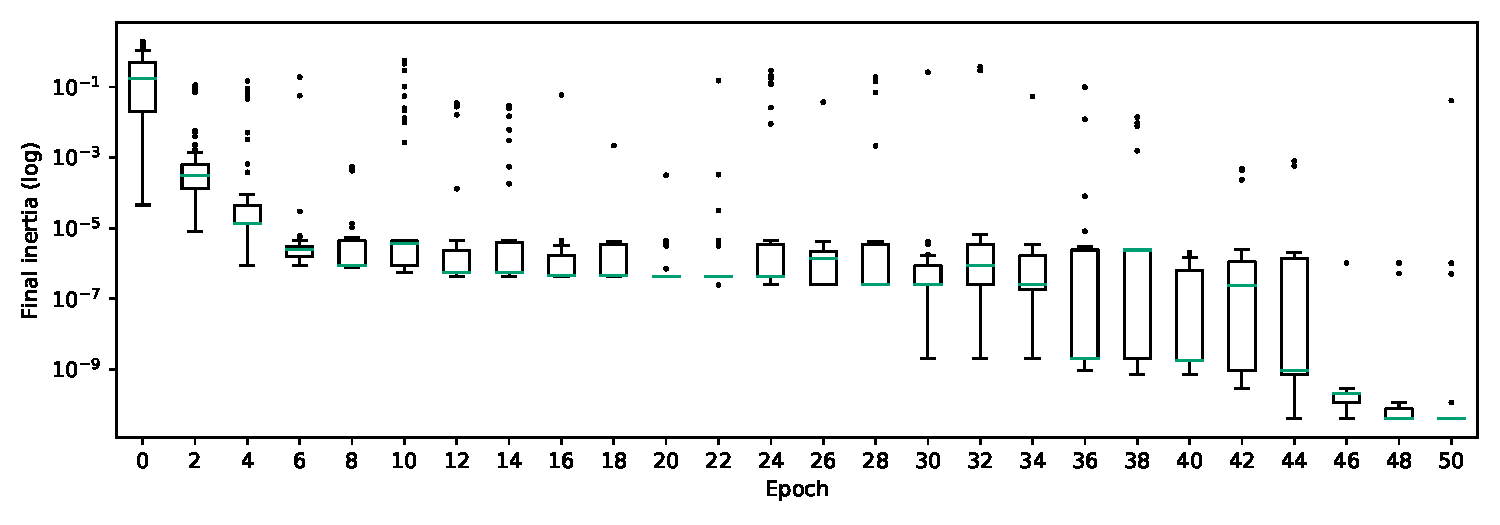
\includegraphics[width=\imgwidth]{Fig7a-1.pdf}
        \\
        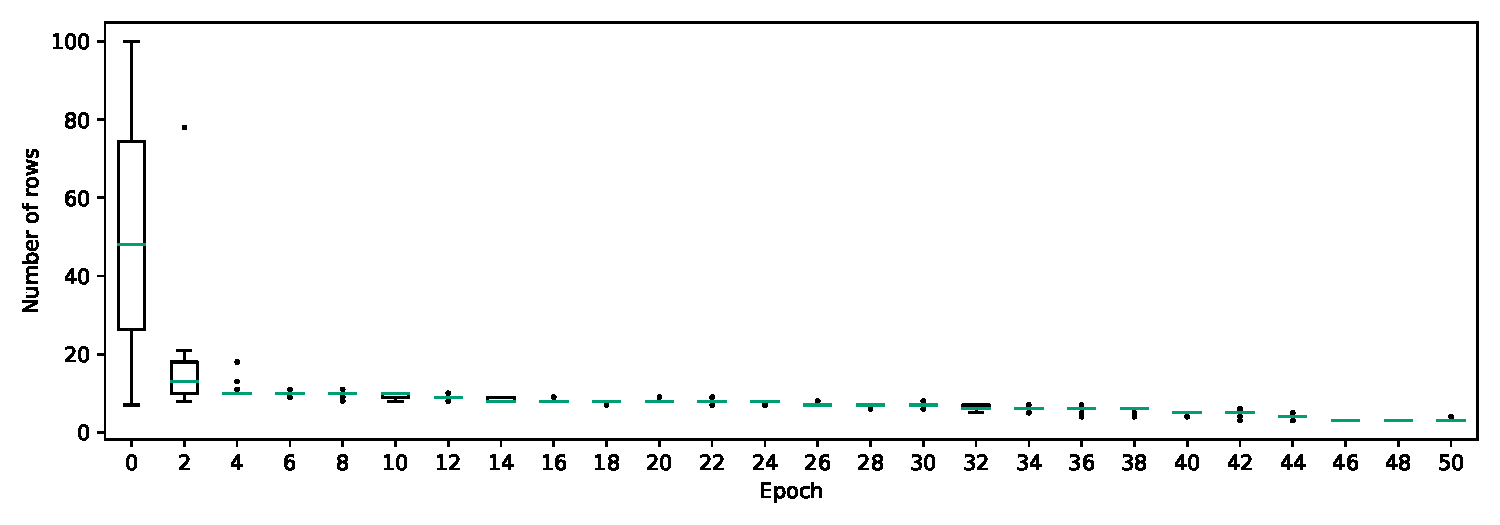
\includegraphics[width=\imgwidth]{Fig7a-2.pdf}
    \end{tabular}
    \caption{%
        Progressions for final inertia and dimension across the first 50
        epochs with \(R~=~(3,100)\).
    }\label{fig:small-inertia-50}
\end{figure}

\begin{figure}[htbp]
    \ContinuedFloat%
    \centering
    \begin{tabular}{c}
        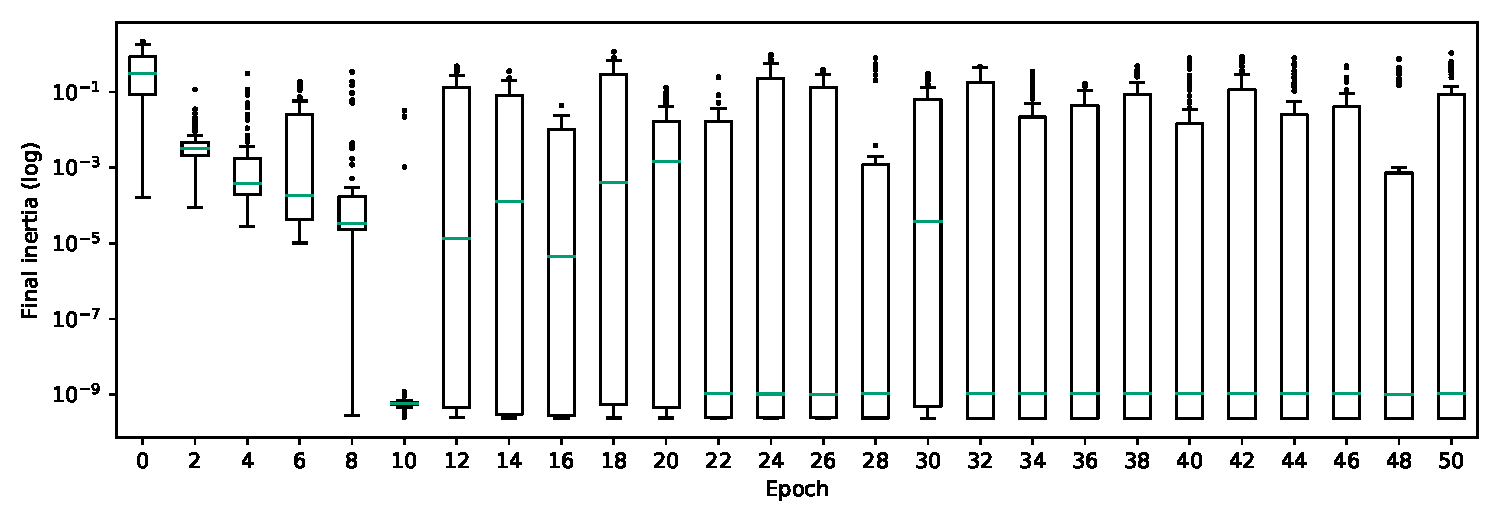
\includegraphics[width=\imgwidth]{Fig7b-1.pdf}
        \\
        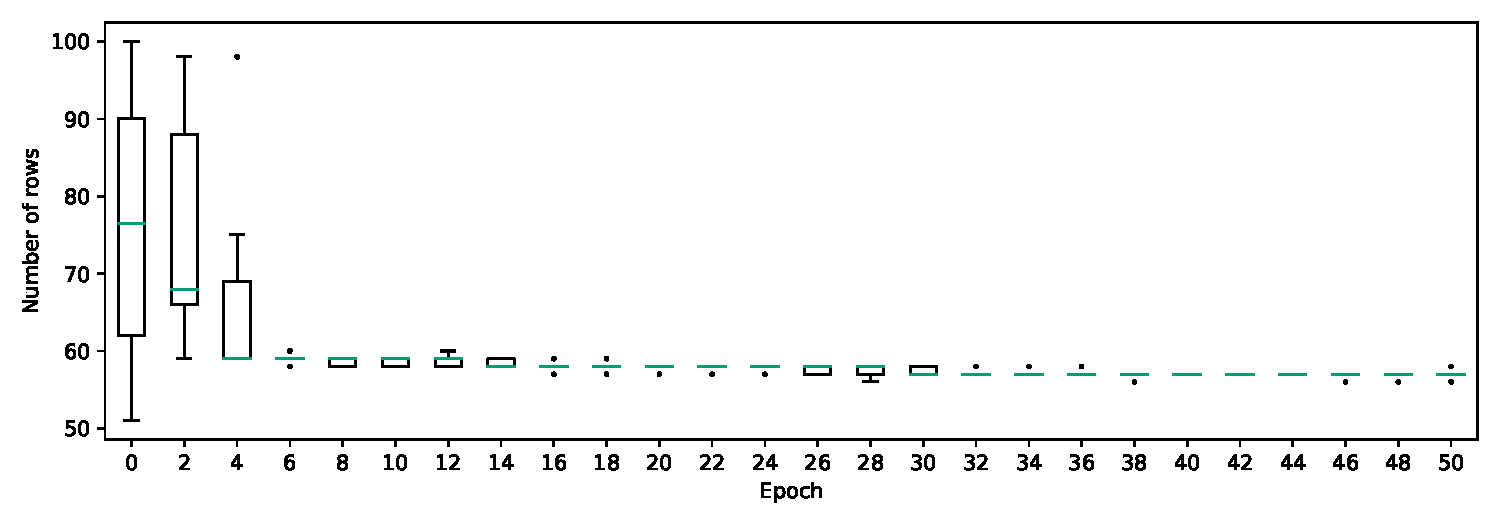
\includegraphics[width=\imgwidth]{Fig7b-2.pdf}
    \end{tabular}
    \caption{%
        Progressions for final inertia and dimension across the first 50 epochs
        with \(R~=~(50,100)\).
    }\label{fig:large-inertia-50}
\end{figure}

However, something that may be seen as unwanted is a compaction of the cluster
centres. Referring to Figure~\ref{fig:small-inertia-inds}, the best and median
individuals show two clusters that are essentially the same point whereas the
worst is a random cloud across the whole of \(\mathcal{U}\) which was found in
the initial population. The kind of behaviour exhibited by the best performing
individuals here occurs in part because it is allowed. There are two immediate
ways in which this allowed: first, that a near-trivial case is included in \(R\)
and, secondly, that the fitness function does nothing to penalise the proximity
of the inter-cluster means, as well as aiming to reduce the intra-cluster means.
This kind of unwanted behaviour highlights a subtlety in how EDO should be used;
that experimentation and rigour are required to properly understand an
algorithm's quality.

\begin{figure}[htbp]
    \centering
    \subfloat[][]{%
        \label{fig:small-inertia-inds}
        \centering
        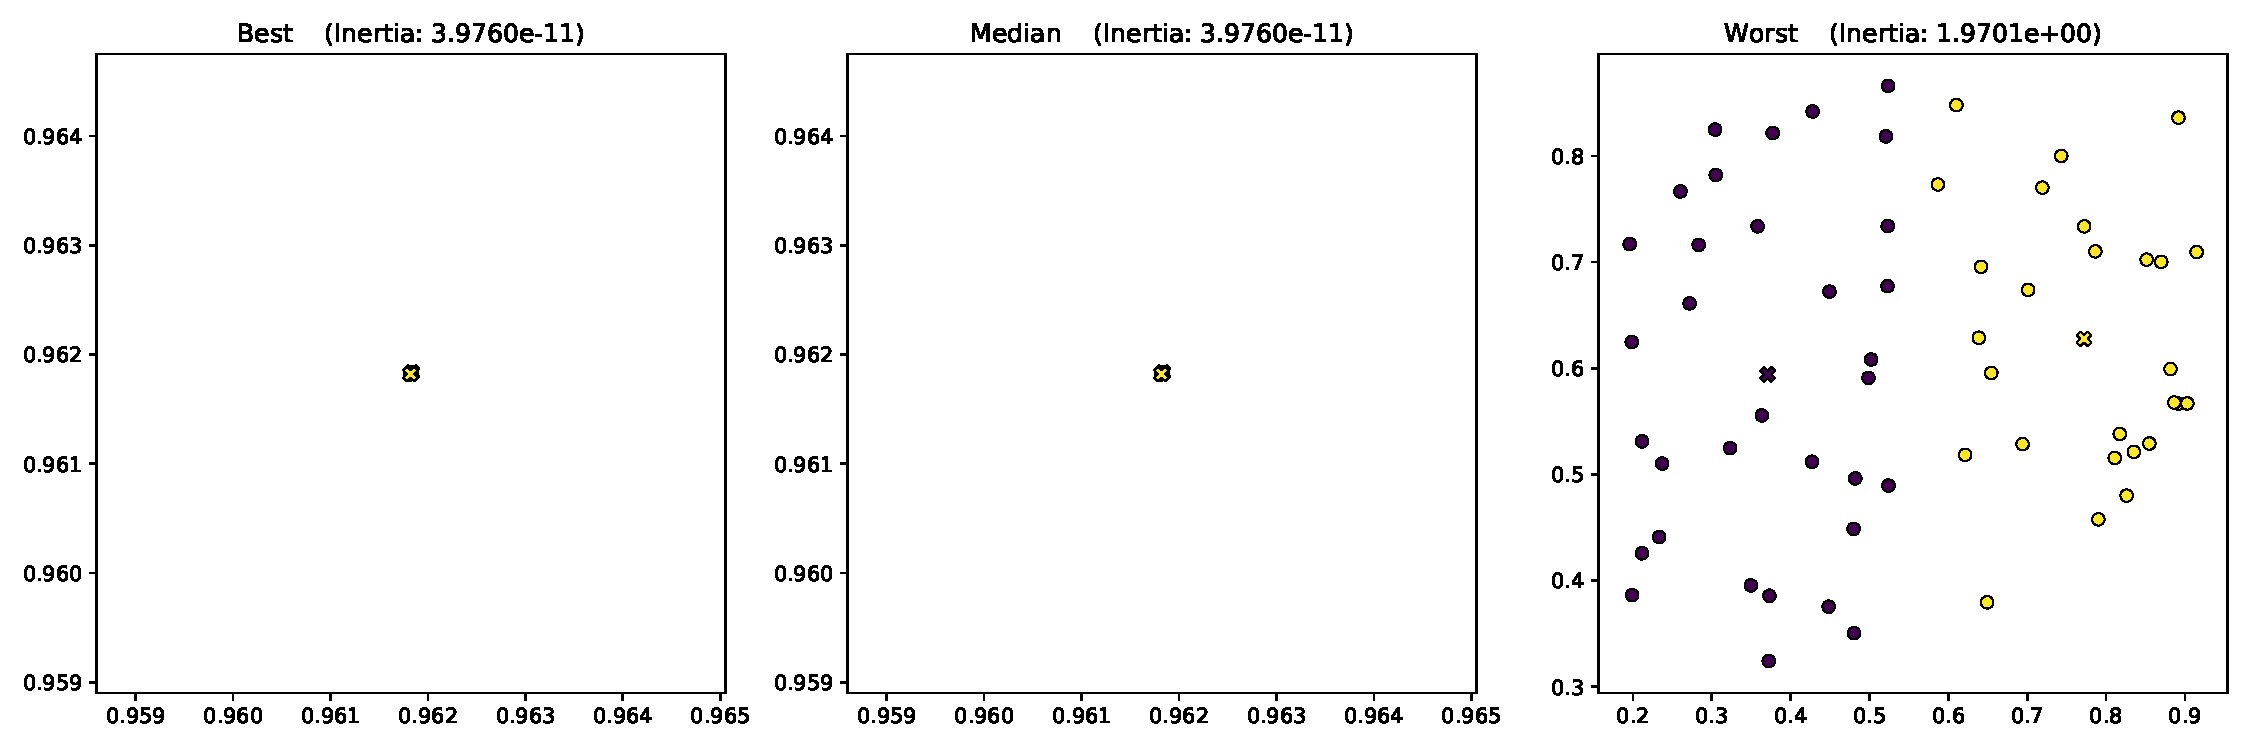
\includegraphics[width=\imgwidth]{Fig8a.pdf}
    }\\

    \subfloat[][]{%
        \label{fig:large-inertia-inds}
        \centering
        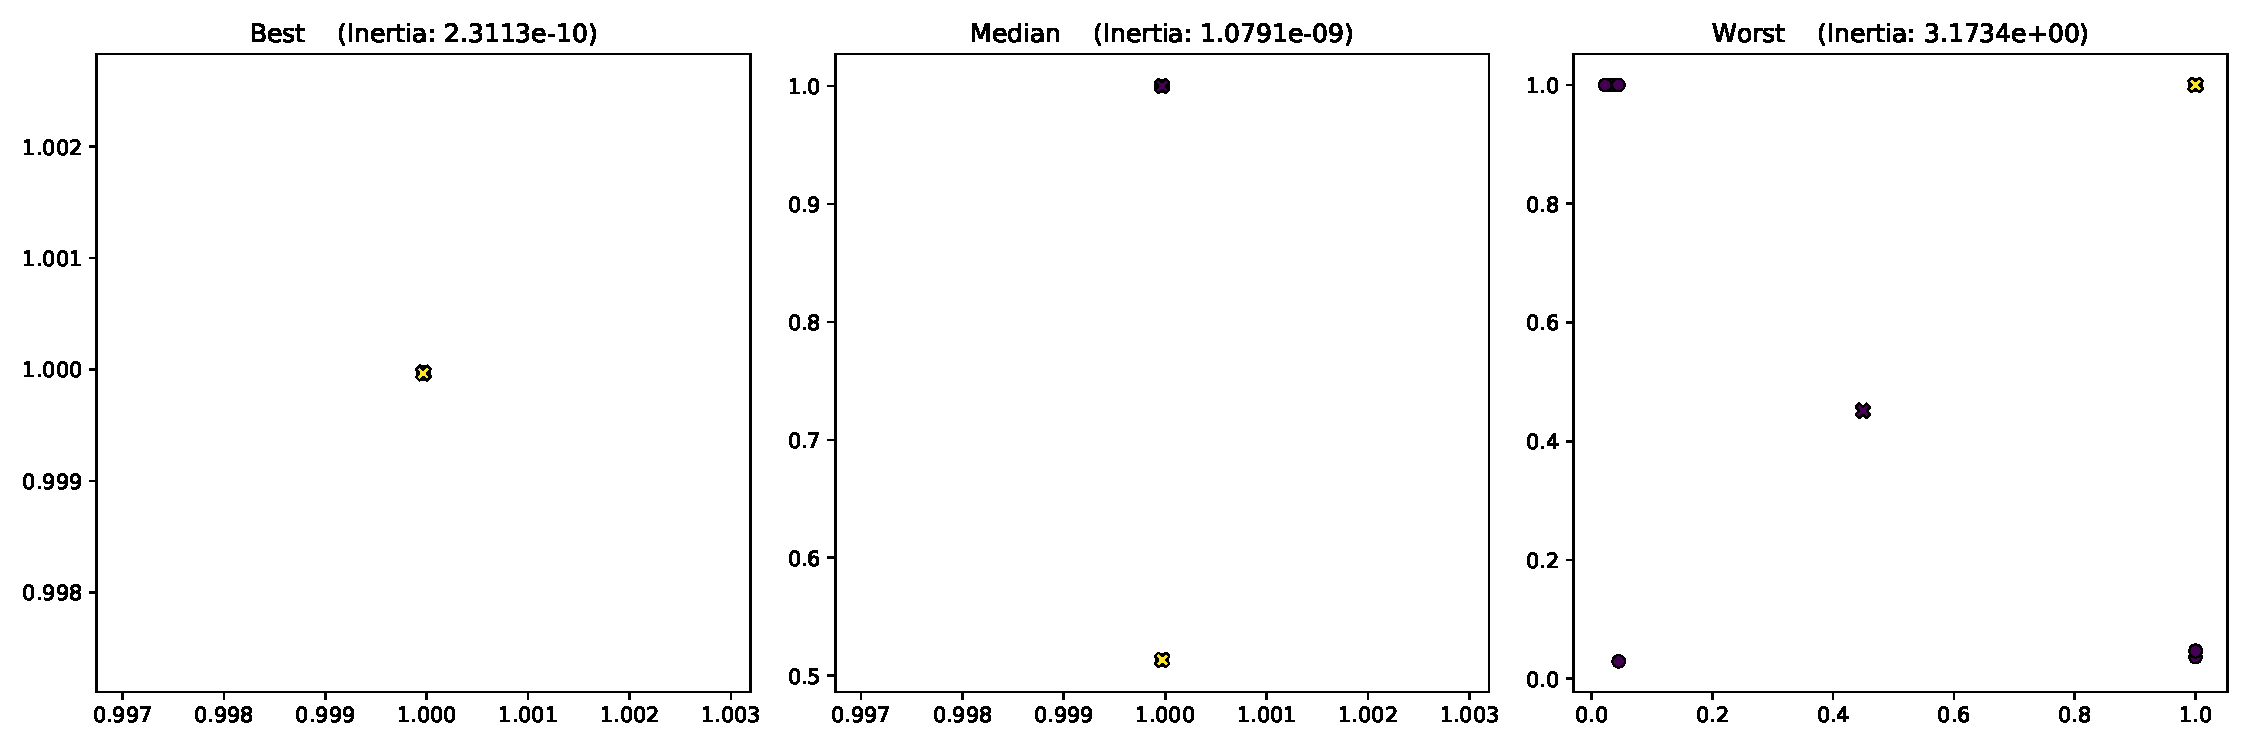
\includegraphics[width=\imgwidth]{Fig8b.pdf}
    }
    \caption[]{%
        Representative individuals based on inertia with:
        \subref{fig:small-inertia-inds} \(R~=~(3,100)\);
        \subref{fig:large-inertia-inds} \(R~=~(50,100)\). Centroids displayed as
        crosses.
    }\label{fig:inertia-inds}
\end{figure}

Hence, consider Figure~\ref{fig:large-inertia-inds} where the individuals have
been generated with the same parameters as previously except with adjusted row
limits, \(R = (50, 100)\), so as to exclude this trivial case. In these trials,
the results are equivalent: the worst performing individuals are without
structure whilst the best-performing individuals display clusters that are dense
about a single point despite the minimum number of rows being increased.
Supposing this was not already a known result, we can see mounting evidence in
favour of this compaction being `optimal' behaviour in a dataset for \(k\)-means
clustering.

However, the fitness function may be addressed still, and more extensive
studying may be done. Indeed, the final inertia could be considered a flawed or
fragile fitness function if it is supposed to evaluate the efficacy of the
\(k\)-means algorithm. Incorporating the inter-cluster spread to the fitness
of an individual dataset would reduce this observed compaction. For instance,
the silhouette coefficient is a metric used to evaluate the appropriateness of a
clustering to a dataset and does precisely that. The silhouette coefficient of a
clustering of a dataset is given by the mean of the silhouette value,
\(S(x)\), of each point \(x \in Z_j\) in each cluster:
\begin{equation}
    \begin{gathered}
        A(x) := \frac{1}{|Z_j| - 1} \sum_{y \in Z_j \setminus \{x\}} d(x, y),
        \\
        B(x) := \min_{k \neq j} \frac{1}{|Z_k|} \sum_{w \in Z_k} d(x, w),
        \\
        S(x) := 
            \begin{cases}
                \frac{B(x) - A(x)}{\max\left\{A(x), B(x)\right\}}
                &\quad \text{if } |Z_j| > 1\\
                0 &\quad \text{otherwise}
            \end{cases}
    \end{gathered}\label{eq:silhouette}
\end{equation}\\

The optimisation of the silhouette coefficient is analogous to finding a dataset
which increases both the intra-cluster cohesion (the inverse of \(A\)) and
inter-cluster separation (\(B\)). Hence, the objective of minimising inertia is
addressed by maximising cohesion. Meanwhile, the additional desire to spread out
the clusters is considered by maximising separation.

Repeating the trials with the same parameters as with inertia, the silhouette
fitness function yields the results summarised in
Figures~\ref{fig:small-silhouette}~and~\ref{fig:large-silhouette}. Irrespective
of row limits, the datasets produced show increased separation from one another
whilst maintaining low values in the final inertia of the clustering as shown in
Figure~\ref{fig:silhouette-inds}. Again, the form of the individual clusters is
much the same. The low values of inertia correspond to tight clusters, and the
tightest clusters are those with a minimal number of points, i.e.\ a single
point. As with the previous example, albeit at a much slower rate, the
preferable individuals are those leading toward this case. That this gradual
reduction in the dimension of the individuals occurs despite adjusting the
fitness function and considering the space which excludes the trivial case
bolsters the claim that the base case is also optimal.

At this point, it should be noted that, due to the nature of the implementation,
any individual from any generation may be retrieved and studied should the final
results be too concentrated on any given case. The summary provided here is one
particular way of studying the body of datasets generated with this method and
this transparency in the history and progression of the proposed method is
something that sets it apart from other methods such as GANs which have a
reputation of providing so-called `black box' solutions.

\addtocounter{figure}{1}
\begin{figure}[htbp]
    \ContinuedFloat%
    \centering
    \begin{tabular}{c}
        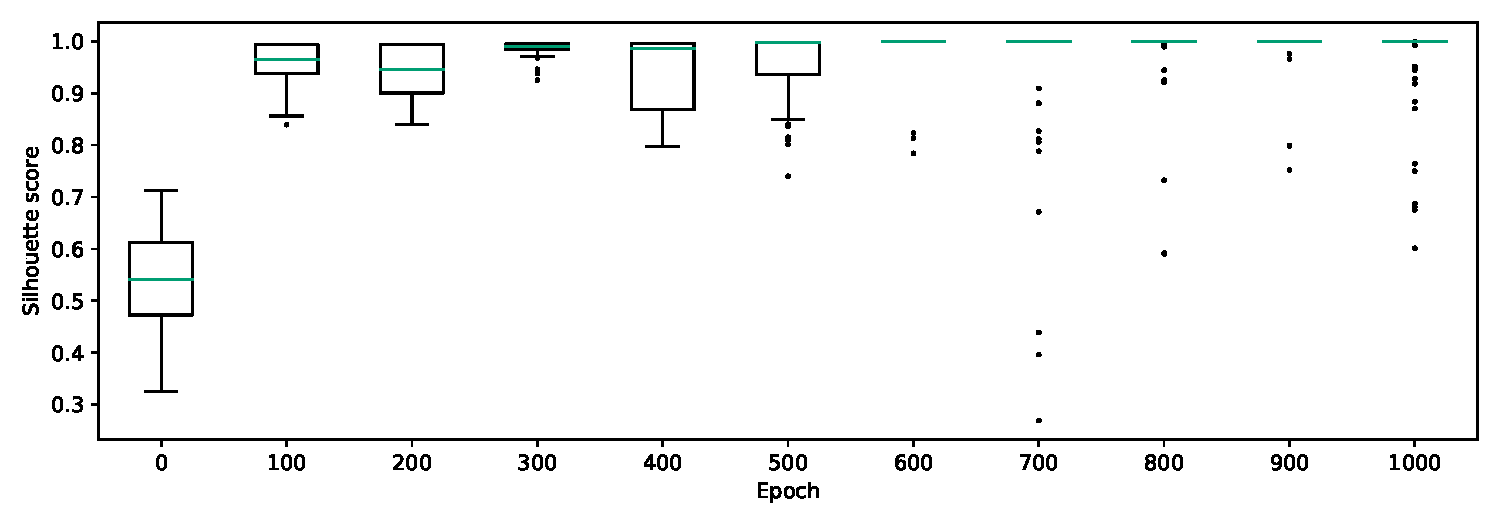
\includegraphics[width=\imgwidth]{Fig9a-1.pdf}
        \\
        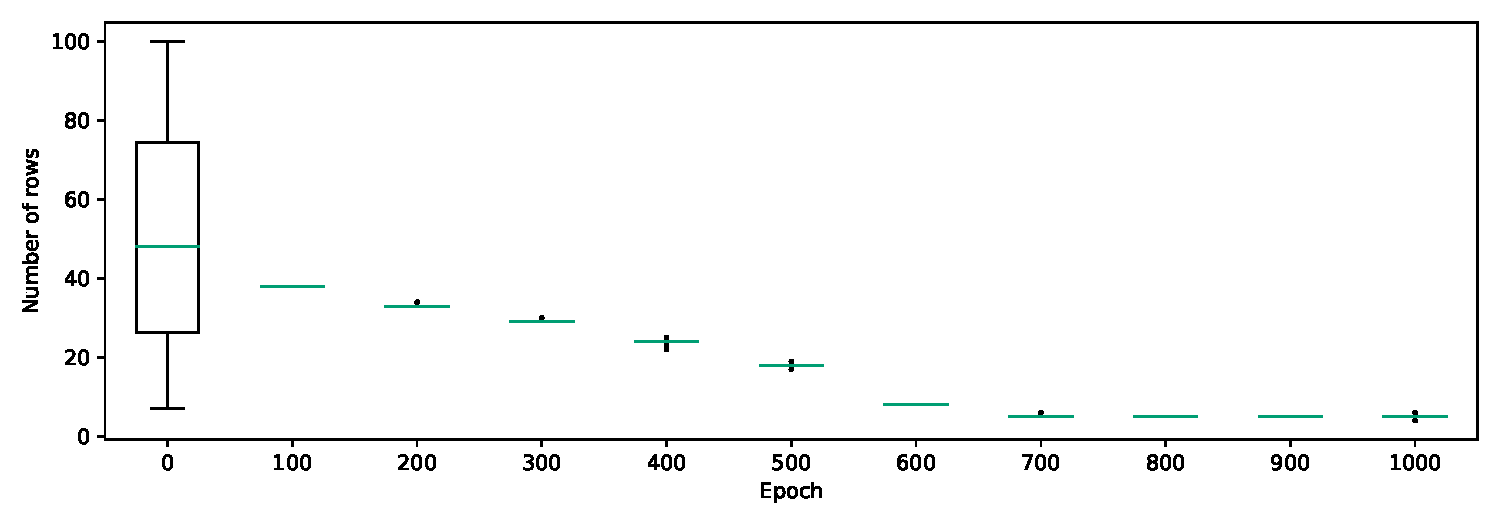
\includegraphics[width=\imgwidth]{Fig9a-2.pdf}
    \end{tabular}
    \caption{%
        Progressions for silhouette and dimension across 1000 epochs at 100
        epoch intervals with \(R~=~(3, 100)\).
    }\label{fig:small-silhouette}
\end{figure}

\begin{figure}
    \ContinuedFloat%
    \centering
    \begin{tabular}{c}
        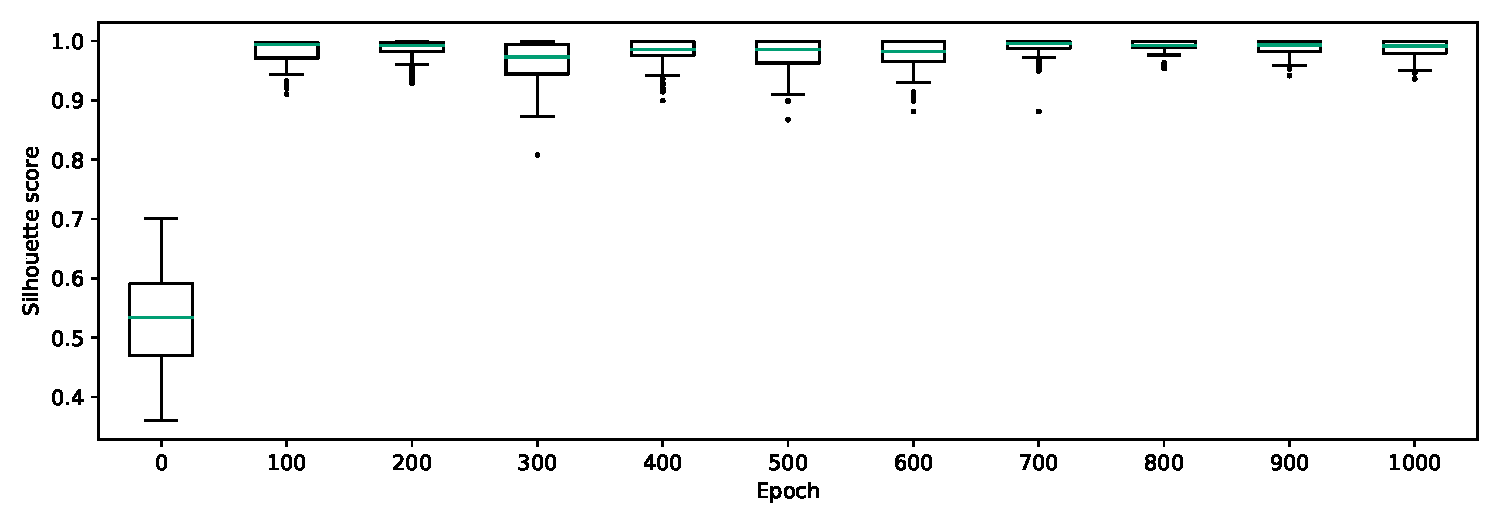
\includegraphics[width=\imgwidth]{Fig9b-1.pdf}
        \\
        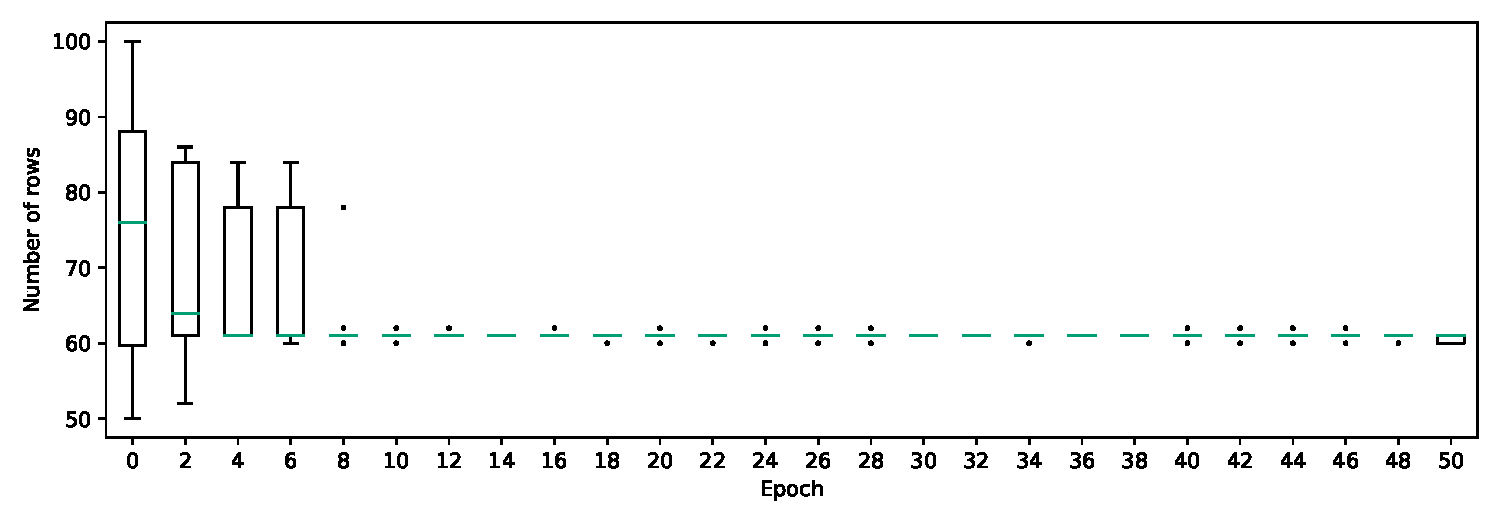
\includegraphics[width=\imgwidth]{Fig9b-2.pdf}
    \end{tabular}
    \caption{%
        Progressions for silhouette and dimension across 1000 epochs at 100
        epoch intervals with \(R~=~(50,100)\).
    }\label{fig:large-silhouette}
\end{figure}

\begin{figure}[htbp]
    \centering
    \subfloat[][]{%
        \label{fig:small-silhouette-inds}
        \centering
        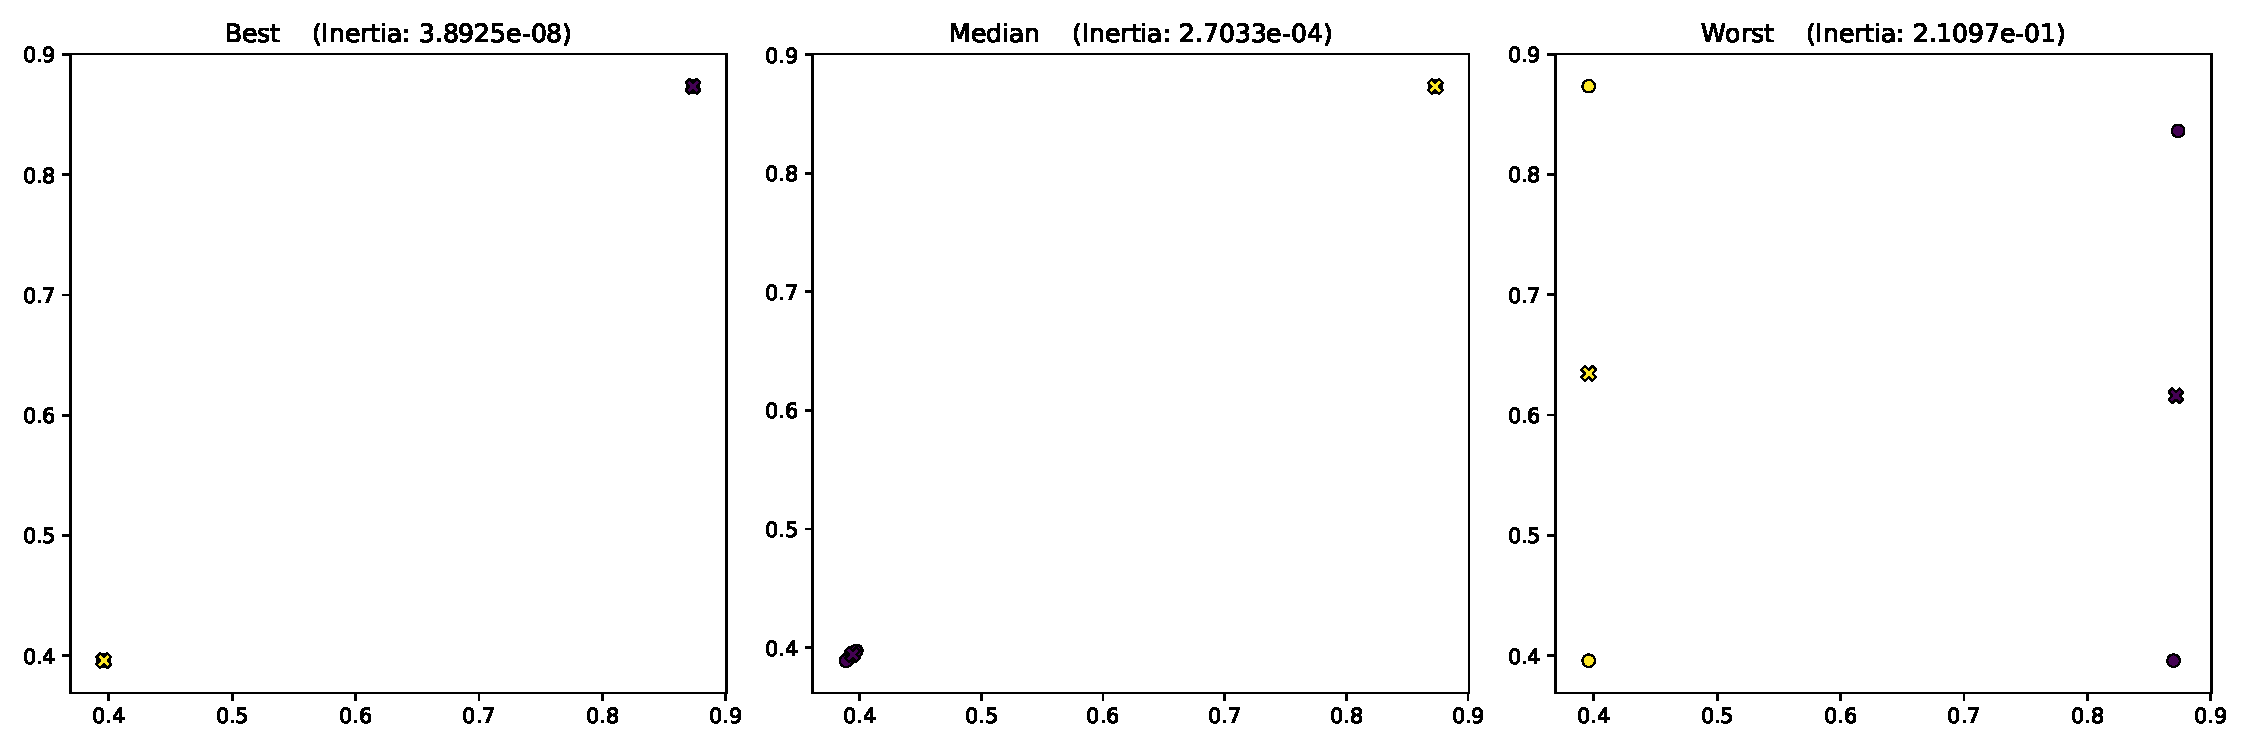
\includegraphics[width=\imgwidth]{Fig10a.pdf}
    }\\

    \subfloat[][]{%
        \label{fig:large-silhouette-inds}
        \centering
        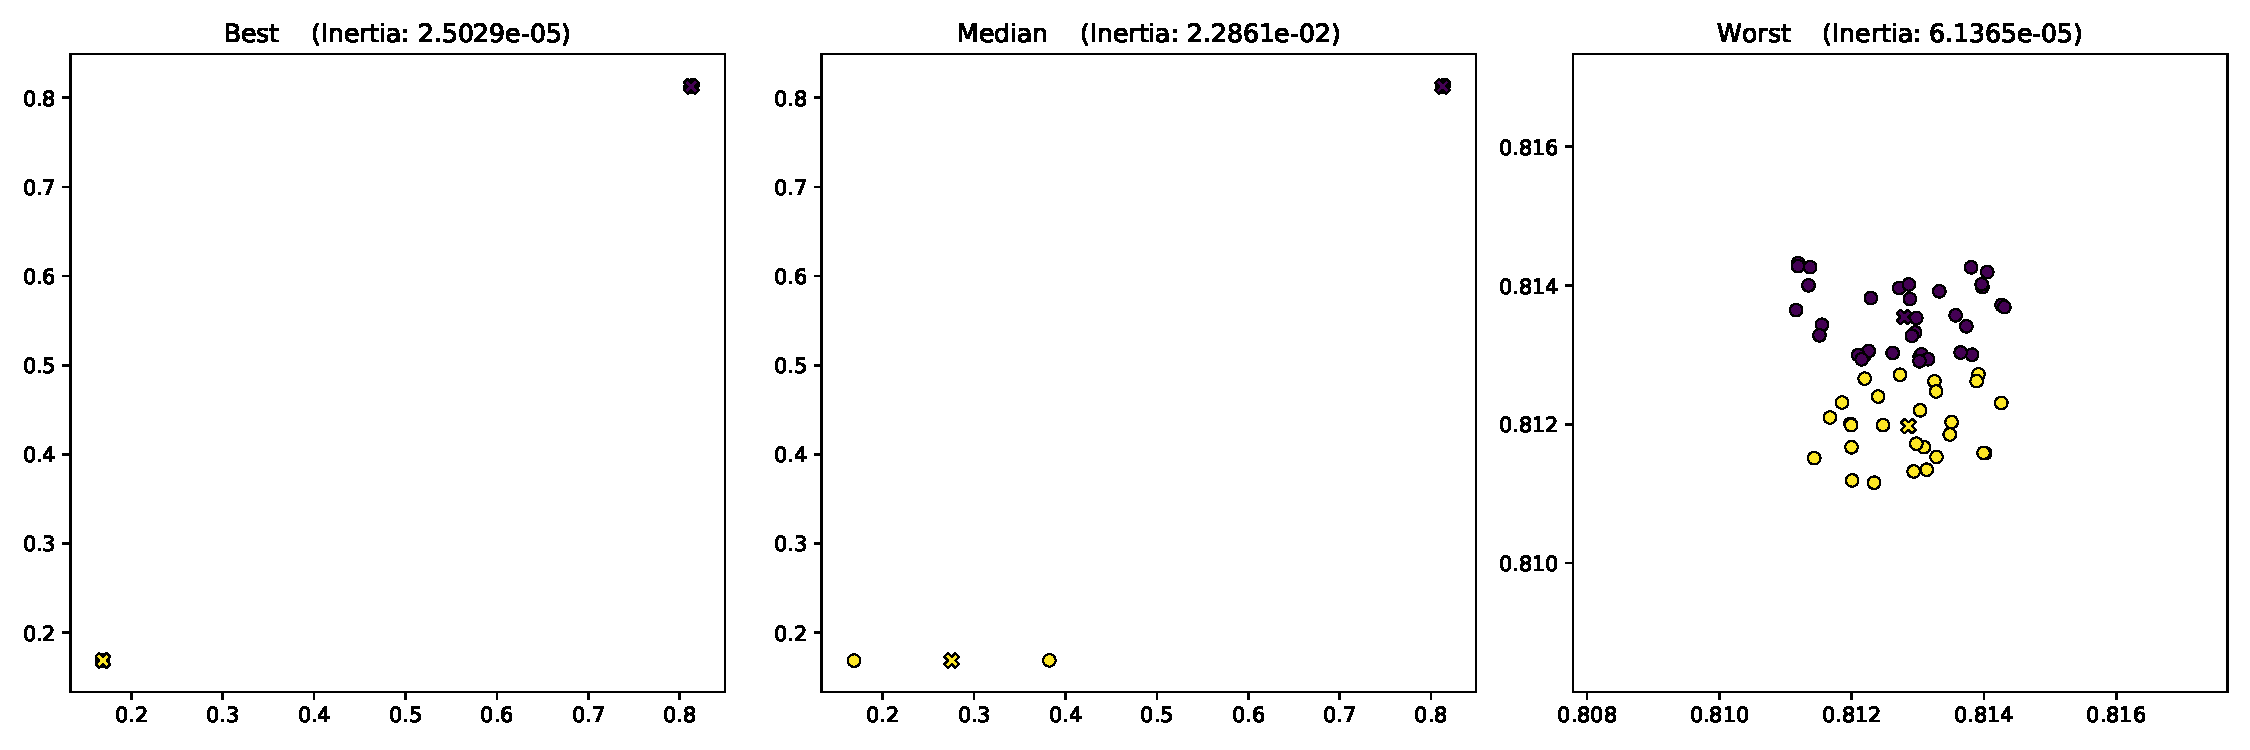
\includegraphics[width=\imgwidth]{Fig10b.pdf}
    }
    \caption[]{%
        Representative individuals based on silhouette with:
        \subref{fig:small-silhouette-inds} \(R~=~(3,100)\);
        \subref{fig:large-silhouette-inds} \(R~=~(50,100)\). Centroids displayed
        as crosses.
    }\label{fig:silhouette-inds}
\end{figure}

\subsection{Comparison with DBSCAN}\label{subsec:dbscan}

The extent of the capabilities EDO holds as a tool to better understand an
algorithm are especially apparent when comparing an algorithm against another
(or set of others) simultaneously. This is done by utilising the freedom of
choice in a fitness function for EDO.\ Consider two algorithms, \(A\) and \(B\),
and some common metric between them, \(g\). Then their similarities and
contrasts can be explored by considering the differences in this metric on the
two algorithms. In terms of EDO, this means using \(f = g_A - g_B\), \(f = g_B -
g_A\) or \(f = \left| g_B - g_A \right|\) as the fitness function. By doing so,
pitfalls, edge cases or fundamental conditions for the method may be
highlighted. Overall, this process allows the researcher to more deeply learn
about the method of interest beyond the traditional method of literature
comparison on a particular example.

Consider the following use case with another clustering algorithm of a different
form, Density Based Spatial Clustering of Applications with Noise (DBSCAN). In
this particular case, the objective is to find datasets for which the method of
interest, \(k\)-means, outperforms its alternative, DBSCAN.\ Here there is no
concept of inertia as DBSCAN is density-based and is able to identify
outliers~\cite{Ester1996}. As such, a valid metric must be chosen. One such
metric is the silhouette score as defined in~(\ref{eq:silhouette}).

In this case, however, an adjustment to the fitness function must be made so as
to accommodate for the condition of the silhouette coefficient that there must
be more than one cluster present. Let \(S_k (X)\) and \(S_D (X)\) denote the
silhouette coefficients of the clustering found by \(k\)-means and DBSCAN
respectively. Then the fitness function is defined to be:
\begin{equation}
    f(X) = 
        \begin{cases}
            S_D (X) - S_k (X), &\quad \text{%
                \begin{tabular}{l}%
                    if DBSCAN identifies two or
                    \\
                    more clusters (inc.\ noise)
                \end{tabular}
            }\\
            \infty &\quad \ \ \text{otherwise.}
        \end{cases}\label{eq:dbscan-fitness}
\end{equation}

There are several remarks to be made here. First, note the order of the
subtraction here as EDO minimises fitness functions by default. Also, \(f\)
takes values in the range \([-2, 2]\) where \(-2\) is the best, i.e.\ \(S_D(X) =
-1\) and \(S_k(X) = 1\). Likewise, 2 is the worst score. Finally, the silhouette
coefficient requires at least two clusters to be present and so if DBSCAN
identifies a single cluster then that individual will be penalised heavily under
this fitness function when, in fact, that clustering may be of high quality. As
such, this fitness function may require adjustment.

It must also be acknowledged that \(k\)-means and DBSCAN share no common
parameters and so direct comparison is more difficult. For the purposes of this
example, only one set of parameters is used but a thorough investigation should
include a parameter sweep in similar, real-world use cases. The parameters being
used are \(k~=~3\) for \(k\)-means, and \(\epsilon~=~0.1,\ MinPoints~=~5\) for
DBSCAN.\ This set was chosen following informal experimentation using the Python
library Scikit-learn~\cite{scikit} to find comparable parameters in the given
search space defined by the EDO parameters used previously with
\(R~=~(50,100)\).

\begin{figure}[htbp]
    \centering
    \begin{tabular}{c}
        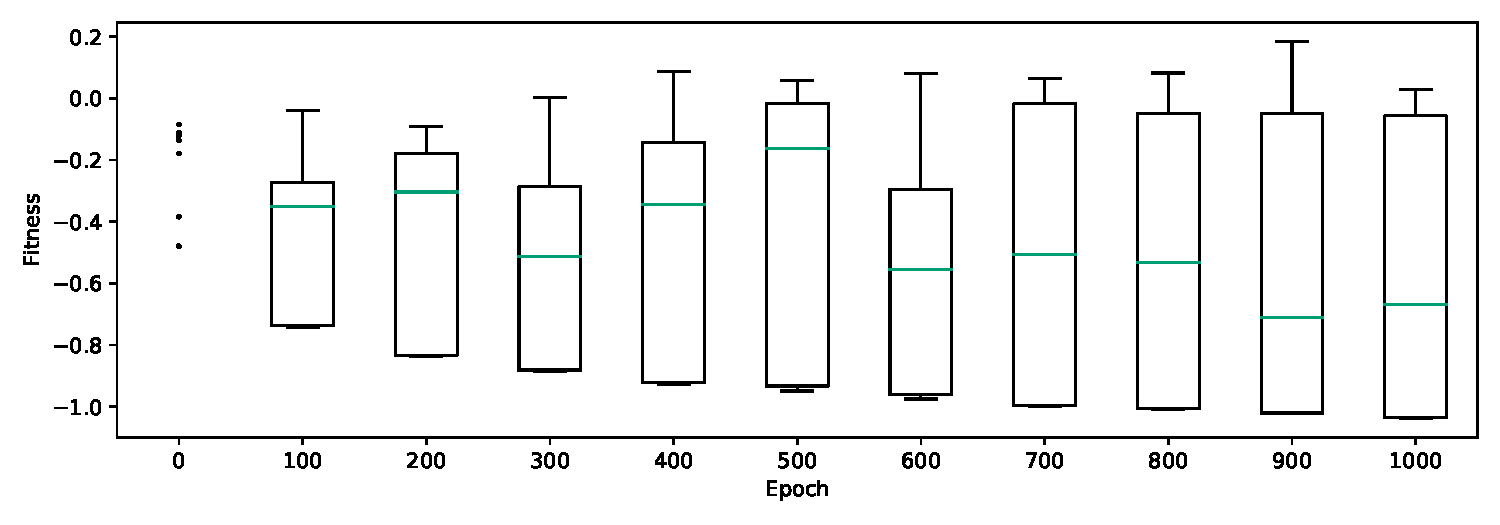
\includegraphics[width=\imgwidth]{Fig11-1.pdf}
        \\
        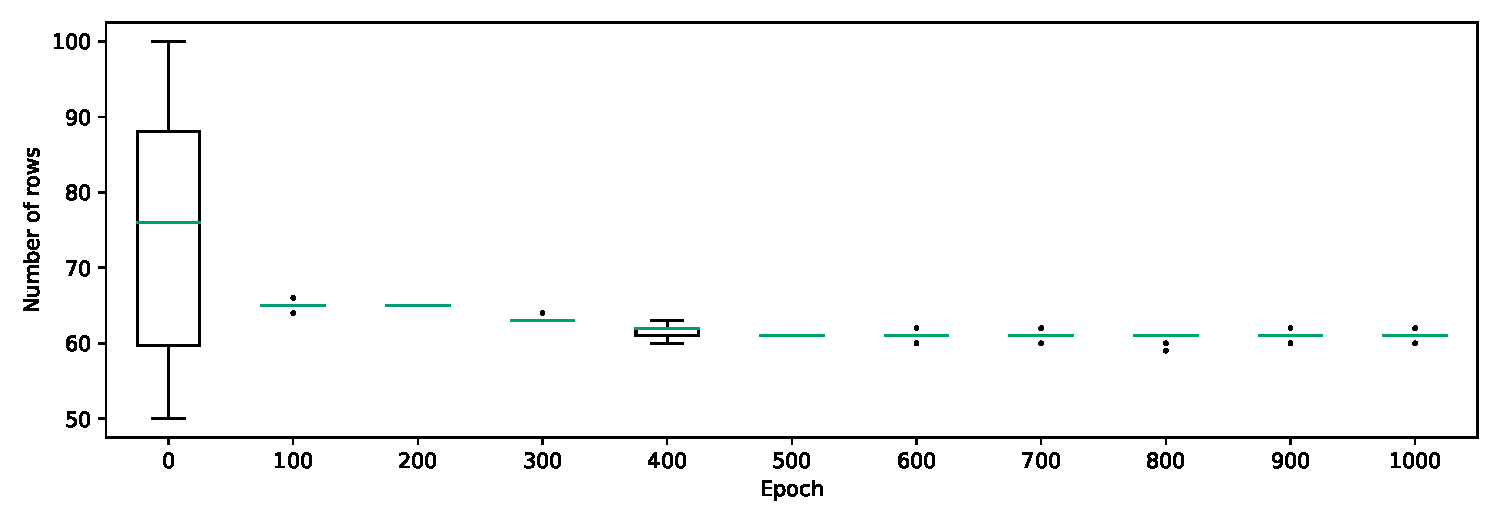
\includegraphics[width=\imgwidth]{Fig11-2.pdf}
    \end{tabular}
    \caption{%
        Progressions for difference in silhouette (\(k\)-means-preferable) and
        dimension across 1000 epochs at 100 epoch intervals.
    }\label{fig:dbscan-silhouette}
\end{figure}

\begin{figure}[htbp]
    \centering
    \subfloat[][]{%
        \label{fig:dbscan-inds-k}
        \centering
        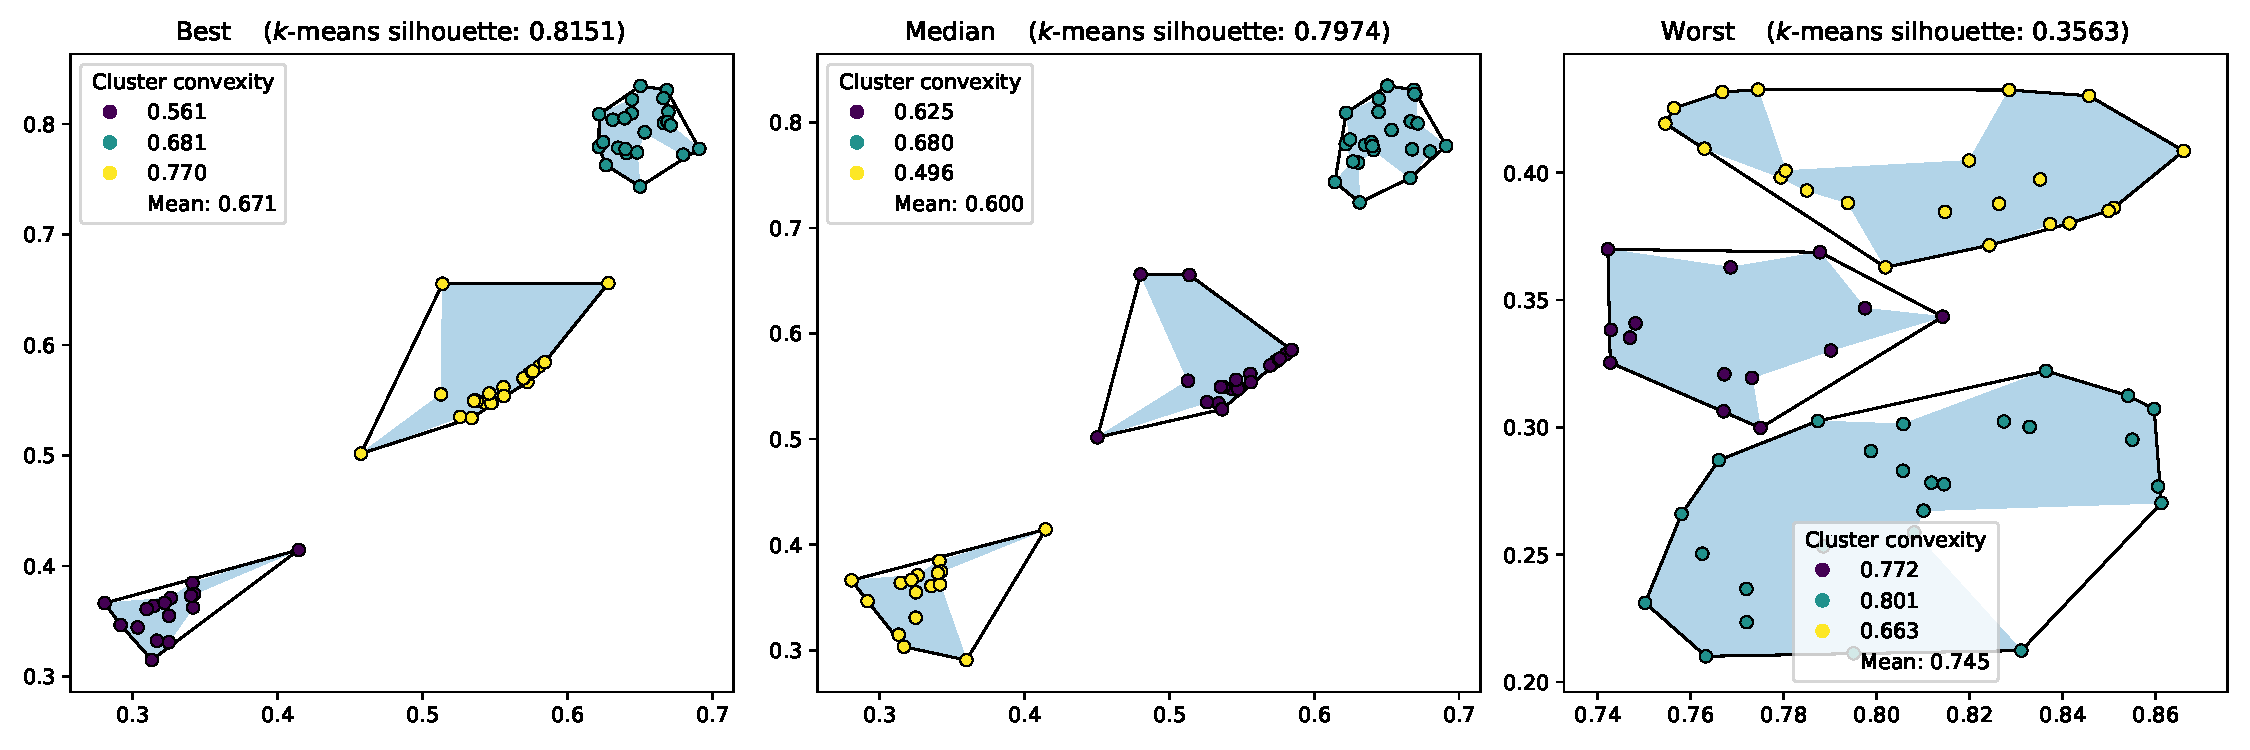
\includegraphics[width=\imgwidth]{Fig12a.pdf}
    }\\
    \subfloat[][]{%
        \label{fig:dbscan-inds-d}
        \centering
        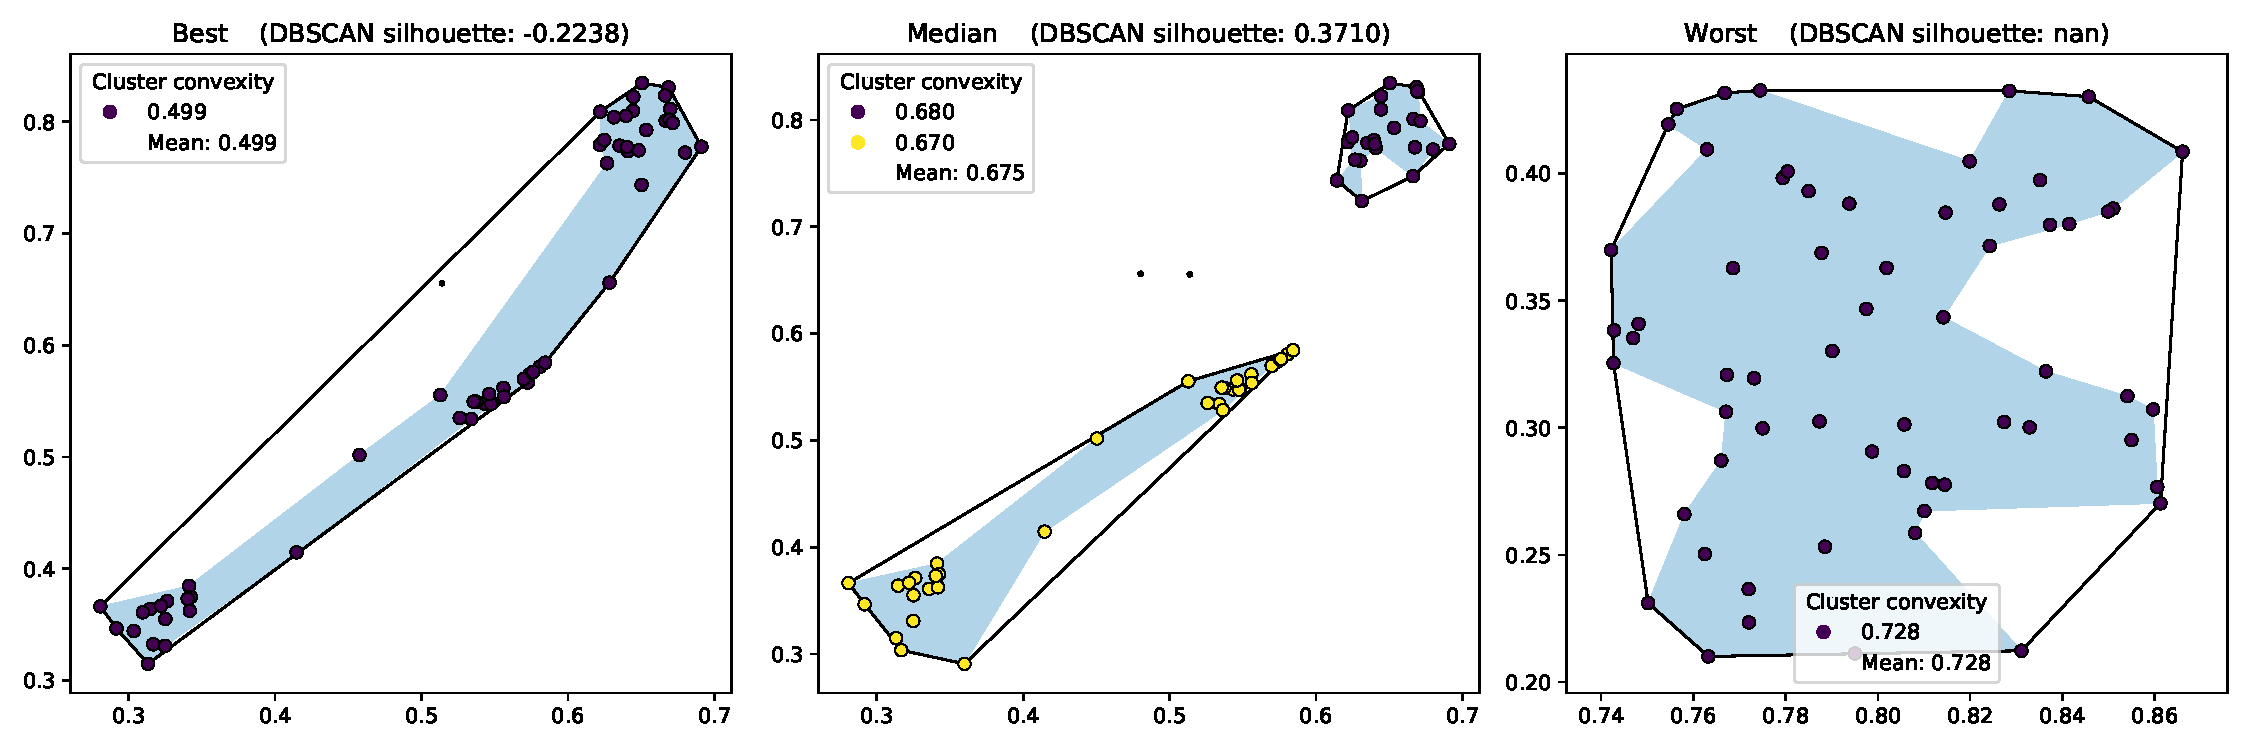
\includegraphics[width=\imgwidth]{Fig12b.pdf}
    }
    \caption[]{%
        Representative individuals from a \(k\)-means-preferable run with
        clustering by: \subref{fig:dbscan-inds-k} \(k\)-means;
        \subref{fig:dbscan-inds-d} DBSCAN.\ Concave and convex hulls illustrated
        by shading and outline respectively. 
    }\label{fig:dbscan-inds}
\end{figure}

Figure~\ref{fig:dbscan-silhouette} shows a summary of the progression of EDO
for this use case. As with the previous examples where \(R~=~(50, 100)\), the
variation in the population fitness is unstable but there is a clear trend of
improvement in the best individual over the course of the run. There is also a
convergence seen in the number of rows a dataset has. The resting dimension
varied across the trials conducted in this work but none exhibited a dramatic
shift toward the lower limit of 50 rows as with previous examples. This is
suggestive of a more competitive environment for individuals where slight
changes to an individual can drastically alter their fitness.

The effect of such changes can be seen in Figure~\ref{fig:dbscan-inds} where
representative individuals are shown for this example. Here, the best performing
individual, when clustered by \(k\)-means, shows three clear and nicely
separated clusters. Note that they are not so tightly packed; again, this
suggests that the route to an optimal individual is less clearly defined. In
contrast, when the same dataset is clustered by DBSCAN a single cluster is found
with a single noise point held within the convex hull of the cluster, i.e.\
there are overlapping clusters (since noise points form a single cluster).
Hence, along with the fact that the larger cluster is widely spread, it follows
that the clustering has a relatively small, negative silhouette coefficient.

Another point of interest here is the convexity of the clusters. A known
condition for the success of \(k\)-means is that the presented clusters are of
roughly equal size and are convex. This is due to the overall objective being to
approximate the centroidal Voronoi tessellation~\cite{Du2006}. Without this
condition, up to the correct choice of \(k\), the algorithm will fail to produce
adequate results for either inertia or silhouette. DBSCAN, on the other hand,
does not have this condition and is able to detect non-convex clusters so long
as they are dense enough. Figure~\ref{fig:dbscan-inds} shows the clustering
found by each method and the respective convex and concave hulls of the clusters
found. The `concave hull' of a cluster is taken to be the \(\alpha\)-shape of
the cluster's data points~\cite{Edelsbrunner1983} where \(\alpha\) is determined
to be the smallest value such that all the points in the cluster are contained
in a single polygon. The convexity of cluster \(Z_j\), denoted
\(\mathcal{C}_j\), is then determined to be the ratio of the area of its concave
hull, \(H_c\), to the area of its convex hull, \(H_v\)~\cite{Sonka1993}:
\begin{equation}
    \mathcal{C}_j := \frac{area(H_c)}{area(H_v)}
\end{equation}

With this definition, it should be clear that a perfectly convex cluster, such
as a single point or line, would have \(\mathcal{C}_j = 1\).

It can be seen that the convexity of the clustering found by \(k\)-means appears
to be higher than that by DBSCAN.\ This was apparent across all trials conducted
in this work and indicates that the condition for convex clusters is being
sought out during the optimisation process. Meanwhile, however, it is not clear
whether the performance of DBSCAN falls owing to its parameters or the method
itself. This is a point where parameter sweeping would prove most useful so as
to determine a crossing point for these two driving forces.

Now, to add to the discussion above, the inverse optimisation should be
considered. That is, using the same parameters, the datasets for which DBSCAN
outperforms \(k\)-means with respect to the silhouette coefficient are to be
investigated. This is equivalent to using \(-f\) as the fitness function
except with the same penalty of \(\infty\) for the case set out
in~(\ref{eq:dbscan-fitness}).

\begin{figure}[htbp]
    \centering
    \begin{tabular}{c}
        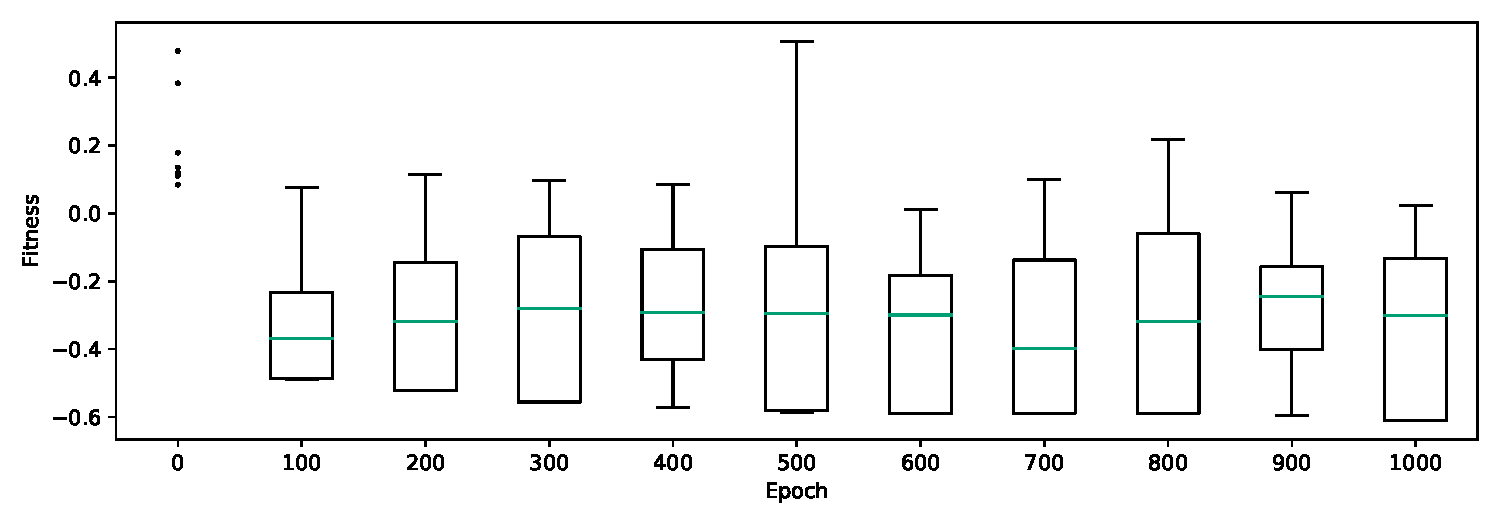
\includegraphics[width=\imgwidth]{Fig13-1.pdf}
        \\
        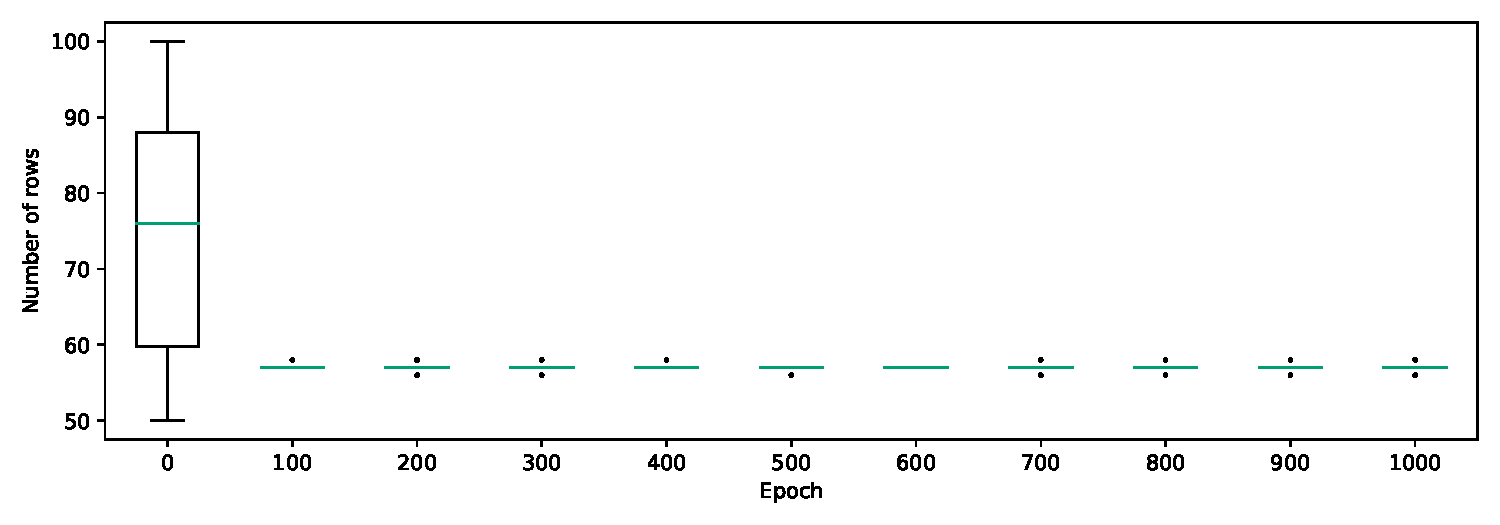
\includegraphics[width=\imgwidth]{Fig13-2.pdf}
    \end{tabular}
    \caption{%
        Progressions for difference in silhouette (DBSCAN-preferable) and
        dimension across 1000 epochs at 100 epoch intervals.
    }\label{fig:negative-prog}
\end{figure}

\begin{figure}[htbp]
    \centering
    \subfloat[][]{%
        \label{fig:neg-inds-k}
        \centering
        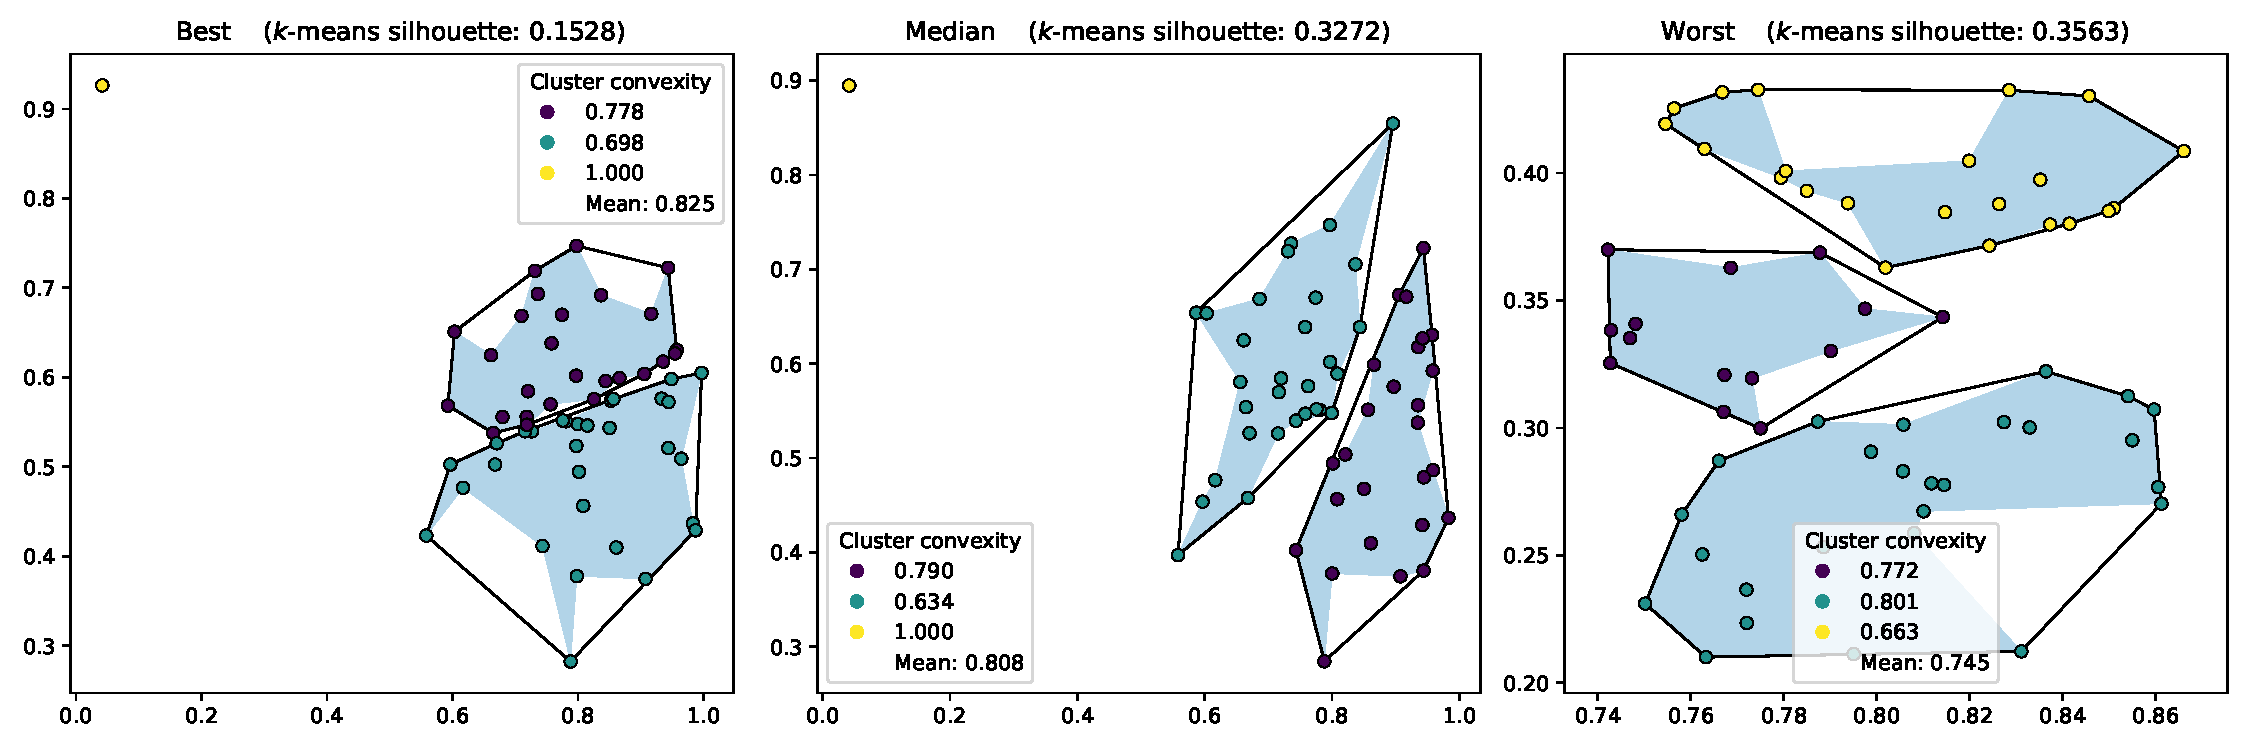
\includegraphics[width=\imgwidth]{Fig14a.pdf}
    }\\
    \subfloat[][]{%
        \label{fig:neg-inds-d}
        \centering
        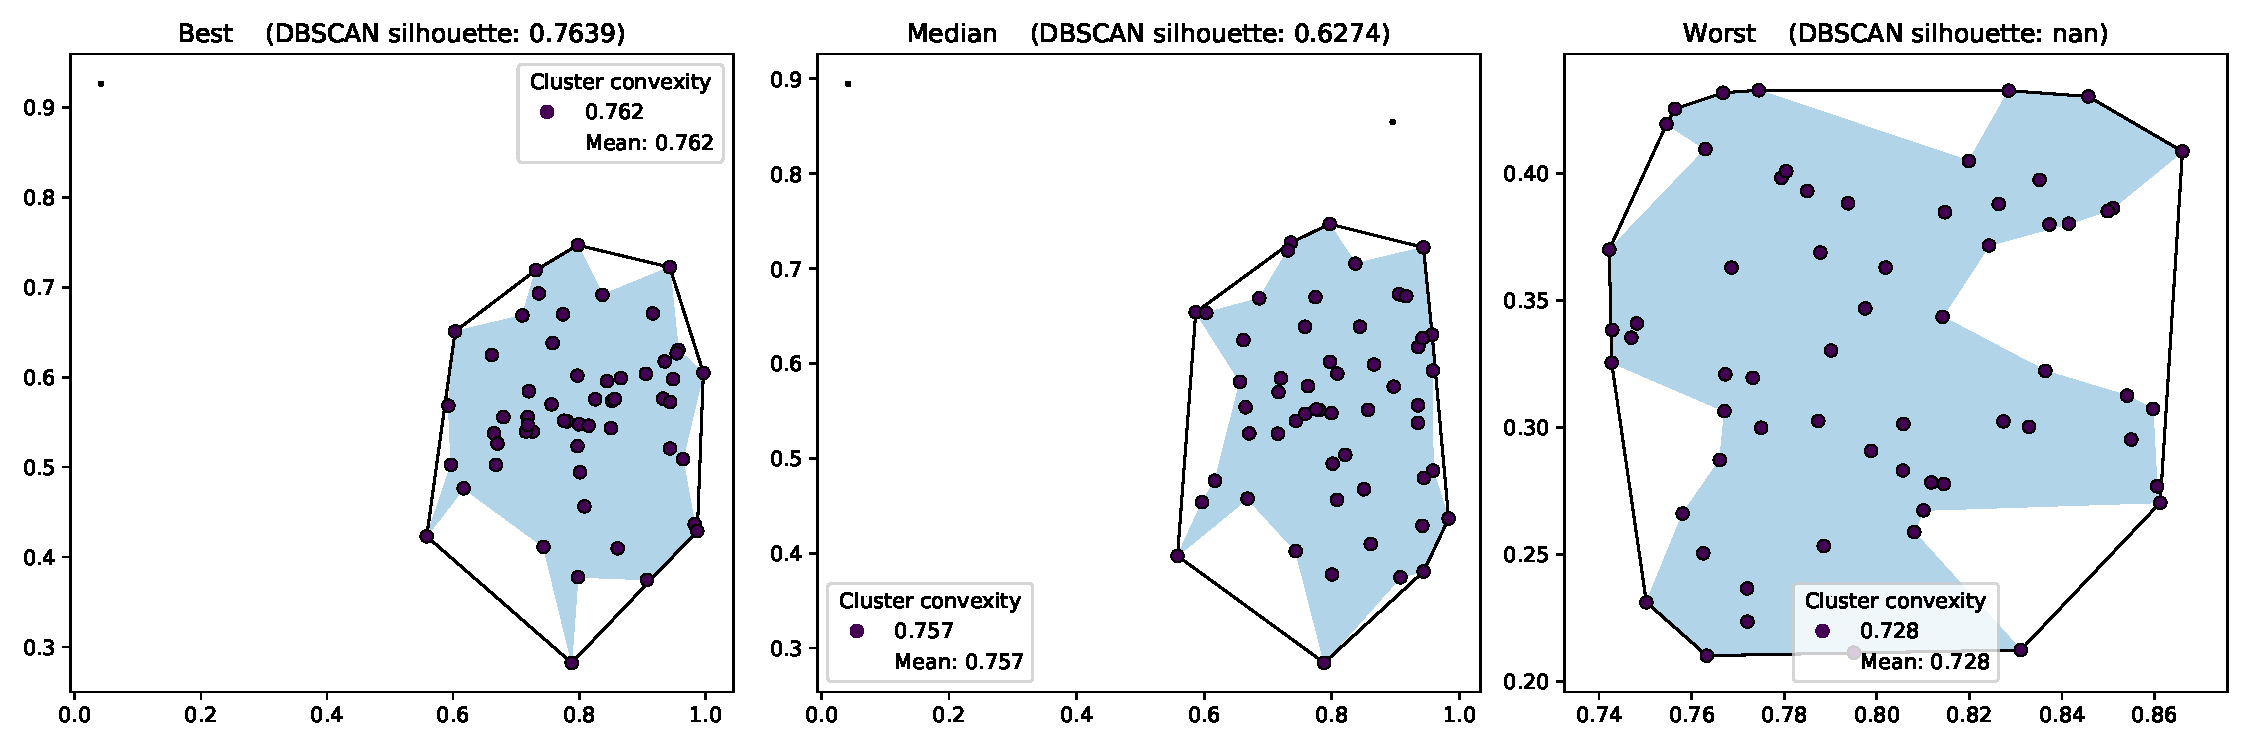
\includegraphics[width=\imgwidth]{Fig14b.pdf}
    }
    \caption[]{%
        Representative individuals from a DBSCAN-preferable run with clustering
        by: \subref{fig:dbscan-inds-k} \(k\)-means; \subref{fig:dbscan-inds-d}
        DBSCAN.\ Concave and convex hulls illustrated by shading and outline
        respectively. 
    }\label{fig:negative-inds}
\end{figure}

Figures~\ref{fig:negative-prog}~and~\ref{fig:negative-inds} show the same
summary as above with the revised fitness function. Inspecting the former, it is
seen that the best fitness found is worse than with the previous example. This,
in part, is due to the fact that \(k\)-means cannot find a clustering with
negative values as no clusters may overlap. It can, however, produce results
with small silhouette scores where the clusters are tightly packed. Hence, the
best fitness score is now \(-1\) whereas the worst is 2, still.

Note in the first two frames of Figure~\ref{fig:neg-inds-k} how \(k\)-means is
forced to split what is evidently a single cluster in two whereas DBSCAN is able
to identify the single cluster and the outlying noise
(Figure~\ref{fig:neg-inds-d}). The proximity of these clusters has then dragged
the silhouette score down for \(k\)-means. Referring to
Figure~\ref{fig:neg-inds-d}, this kind of behaviour is certainly preferable for
DBSCAN under these parameters: the beginning individuals are likely random
clouds (as seen in the rightmost two frames of the figure) and the simplest step
toward a fit dataset is one that maintains that vaguely dense body with minimal
noise points far from it.

As has already been stated, the software implementation of the EDO method
has been produced in line with the best practices of open source software
development and reproducible research. In aid of this, all of the source code
used in these examples (including to create the figures) has been archived
under the DOI
\href{https://doi.org/10.5281/zenodo.3492236}{10.5281/zenodo.3492236}.
Likewise, all of the data produced to support this case study have been archived
under the DOI
\href{https://doi.org/10.5281/zenodo.3492228}{10.5281/zenodo.3492228}.


